\documentclass[a4paper]{book}

%%% INICIO DEL PREÁMBULO %%%

\usepackage[utf8]{inputenc}
\usepackage[greek,spanish,es-tabla,es-nodecimaldot,es-noindentfirst]{babel}
\usepackage{babelbib}
\usepackage{nccmath}
\usepackage{amsthm}
\usepackage{lipsum}
\usepackage{tcolorbox}
\usepackage[thicklines]{cancel}
\usepackage{mathtools}
\usepackage{amssymb}
\usepackage{amsmath}
\usepackage{caption}
\usepackage{subcaption}
\usepackage{color}
\usepackage{verbatim}
\usepackage{enumerate}
\usepackage{geometry}
\geometry{a4paper,left=35mm,right=35mm,top=15mm,bottom=15mm}
\usepackage{isotope}
\usepackage{maybemath}
\usepackage{upgreek}
\usepackage{wasysym}
\usepackage[italic]{hepparticles}
\usepackage{subdepth}
\usepackage{siunitx}
\sisetup{
	mode 			= text,
	parse-units 	= false
}
\usepackage{physics}
\usepackage{braket}
\usepackage{tensor}
\usepackage{chemformula}
\usepackage{tikz}
\usepackage{url}
\usepackage{listings}
\usepackage{multirow}
\usepackage{multicol}
\usepackage[colorlinks=true]{hyperref}
\hypersetup{
	citecolor = blue,
	linkcolor = blue,
	urlcolor = blue,
	pdfauthor = {Javier Rodrigo López}
}
\usepackage{eso-pic}

% tikz
\usepackage{tikz} \usetikzlibrary{fit,babel,shapes,arrows,patterns,positioning,calc,decorations.pathmorphing,decorations.markings}
\tikzstyle{block} = [draw, fill=white, rectangle,
minimum height=3em, minimum width=6em]
\tikzstyle{sum} = [draw, fill=white, circle, node distance=1cm]
\tikzstyle{input} = [coordinate]
\tikzstyle{output} = [coordinate]
\tikzstyle{pinstyle} = [pin edge={to-,thin,black}]
\tikzset{
	block/.style = {draw, fill=white, rectangle, minimum height=3em, minimum width=3em},
	tmp/.style  = {coordinate},
	sum/.style= {draw, fill=white, circle, node distance=1cm},
	input/.style = {coordinate},
	output/.style= {coordinate},
	pinstyle/.style = {pin edge={to-,thin,black}}
}

\usepackage[oldvoltagedirection]{circuitikz}
\usepackage{pdflscape}

% Títulos
\usepackage{titlesec}
\titleformat{\section}{\normalfont\Large\bfseries}{\thesection}{1em}{}[{\titlerule[0.8pt]}]
% \renewcommand{\thesubsection}{\arabic{chapter}.\arabic{section}.\Alph{subsection}}
\titleformat{\subsubsection}{\normalfont\normalsize\bfseries}{\thesubsubsection}{1em}{}[{\titlerule[0.05pt]}]
\titlespacing{\section}{0pt}{2\parskip}{\parskip}
\titlespacing{\subsection}{0pt}{\parskip}{0pt}
\titlespacing{\subsubsection}{0pt}{\parskip}{0pt}

% Numeración de secciones
\setcounter{tocdepth}{2}
\setcounter{secnumdepth}{2}

% Figuras y descripciones
\renewcommand{\thefigure}{\arabic{figure}}
\renewcommand{\thesubfigure}{\Alph{subfigure}}
\captionsetup[figure]{labelfont={bf},name={Figura},labelsep=period}
\numberwithin{figure}{chapter}
\numberwithin{equation}{chapter}

% Enumerations
\newcounter{myenumi}
\renewcommand{\themyenumi}{\alph{myenumi})}
\newenvironment{myenumerate}{\setlength{\parindent}{0pt}\setcounter{myenumi}{0}\renewcommand{\item}{\par\refstepcounter{myenumi}\makebox[1.3em][l]{\themyenumi}}}{\par\bigskip\noindent\ignorespacesafterend}

% Own environments
\newenvironment{nota}{\underline{\textbf{NOTA:}} }{}
\newenvironment{caja}{\begin{tcolorbox}[colback = white, sharp corners, boxrule = 1 pt]}{\end{tcolorbox}}
\newtheorem*{conclusion}{Conclusión}
\newtheorem{teorema}{Teorema}
\newtheorem{definicion}{Definición}

% Para una bonita portada
\usepackage{wallpaper}
\usepackage{titling}
\usepackage{fancyhdr}
\pagestyle{fancy}
\setlength{\droptitle}{-10cm}
\renewcommand{\chaptermark}[1]{%
	\markboth{#1}{}}
\renewcommand{\sectionmark}[1]{%
	\markright{}}
\fancyhf{}
\fancyhead[LE,RO]{\bfseries\thepage} \fancyhead[LO]{\bfseries\rightmark} \fancyhead[RE]{\bfseries\leftmark} \renewcommand{\headrulewidth}{0pt} \renewcommand{\footrulewidth}{0pt} \addtolength{\headheight}{15pt}
\fancypagestyle{plain}{%
	\fancyhead{}
	\renewcommand{\headrulewidth}{0pt}
}

% Organización del texto
\newcommand{\formula}[1]{\vspace{13 pt}\noindent \textbf{\underline{#1}}}
\newcommand{\subtext}[1]{_{\text{#1}}}

% Unidades y utilidades varias
\renewcommand{\S}{\operatorname{S}}
\newcommand{\dB}{\operatorname{dB}}
\newcommand{\dBW}{\operatorname{dBW}}
\newcommand{\dBm}{\operatorname{dBm}}
\newcommand{\Hz}{\operatorname{Hz}}
\newcommand{\s}{\operatorname{s}}
\newcommand{\A}{\operatorname{A}}
\newcommand{\V}{\operatorname{V}}
\newcommand{\ohm}{\,\Omega}
\newcommand{\Pa}{\operatorname{Pa}}
\newcommand{\W}{\operatorname{W}}
\newcommand{\I}{\operatorname{I}}
\newcommand{\C}{\operatorname{C}}
\newcommand{\K}{\operatorname{K}}
\newcommand{\m}{\operatorname{m}}
\newcommand{\mm}{\operatorname{mm}}
\newcommand{\rad}{\operatorname{rad}}
\newcommand{\mol}{\operatorname{mol}}
\newcommand{\J}{\operatorname{J}}
\newcommand{\kg}{\operatorname{kg}}
\newcommand{\incremento}{\Delta}
\newcommand{\psus}{\, \ldots \,}
\newcommand{\mcm}{\operatorname{mcm}}
\newcommand{\MCD}{\operatorname{MCD}}
\renewcommand{\sin}{\sen}
\renewcommand{\arcsin}{\arcsen}
\renewcommand{\arctan}{\arctg}
\renewcommand{\min}{\operatorname{mín}}

\DeclarePairedDelimiter\evaluat{.}{\rvert}

% Vectores
\usepackage[c]{esvect}
\renewcommand{\vec}[1]{\vv{{#1}}}
\newcommand{\proy}[2]{\operatorname{proy}_{\vec{#2}}\vec{#1}}
\newcommand{\antiparallel}{\downharpoonleft \! \upharpoonright}
\newcommand{\parallelvec}{\upharpoonleft \! \upharpoonright}

% Espaciado
\usepackage{enumitem}
\setlist{before={\parskip=3pt}, after=\vspace{\baselineskip}}
\setlength{\parindent}{0pt}
\setlength{\parskip}{0.5em}

% Estadística
\DeclareMathOperator{\Var}{Var}
\DeclareMathOperator{\Cov}{Cov}
\renewcommand{\var}{\sigma ^2}
\DeclareMathOperator{\B}{B}
\DeclareMathOperator{\BN}{BN}
\DeclareMathOperator{\Geo}{Geo}
\DeclareMathOperator{\Poisson}{Poisson}
\DeclareMathOperator{\U}{U}
\DeclareMathOperator{\Exp}{Exp}
\DeclareMathOperator{\N}{N}
\DeclareMathOperator{\Mult}{Mult}
\newcommand{\TF}[1]{\mathrm{TF} \left\lbrace \left. #1 \right\rbrace \right.}
\newcommand{\probCond}[2]{P \left( #1 \: \middle\vert\:  #2 \right) }

% Electromagnetismo y Ondas
\newcommand{\errorGrave}{\textbf{FG!!!}}
\newcommand{\mas}{M.A.S.}
\newcommand{\mcu}{M.C.U.}
\newcommand{\ed}{E.D.}
\newcommand{\edmas}{E.D. del M.A.S.}
\usepackage{esint}

% Señales y Sistemas
\renewcommand{\H}{H}

% Circled number
\newcommand{\circledNumber}[1]{\raisebox{.9pt}{\textcircled{\raisebox{-.9pt}{#1}}}}

% Footnotes
% \renewcommand{\thefootnote}{\fnsymbol{footnote}}

% Ejemplo
\newcounter{elejemplo}
\newcommand{\ejemplo}[2]{
	\refstepcounter{elejemplo}
	\begin{center}
		\fbox{\begin{minipage}{0.85\linewidth}
			\textbf{Ejemplo \arabic{elejemplo}.} #1
			\begin{center}
				\underline{\textbf{Solución}}
			\end{center}
			#2
		\end{minipage}}
	\end{center}
}

% Repeticiones
\usepackage{forloop}
\newcommand{\repvec}[3]{
	\foreach \uwu in {1,...,#2}
		{\vec{#1}_{\uwu} ,}
	\, \ldots \, , \vec{#1}_{#3}
}
\newcommand{\rep}[3]{
	\foreach \uwu in {1,...,#2}
		{#1_{\uwu} ,}
	\, \ldots \, , #1_{#3}
}
\newcommand{\repinf}[3]{
	\foreach \uwu in {#2,...,#3}
		{#1_{\uwu} ,}
	\, \ldots
}

%%% FIN DEL PREÁMBULO %%% % Se incluye el preámbulo

\renewcommand{\vec}[1]{\mathbf{#1}} % Redefinición de vectores para adecuarse a la notación de negrita usada en esta asignatura.

\title{\Huge Estadística y Procesos Estocásticos\\
\Large Apuntes de clase}
\author{Javier Rodrigo López \thanks{E-mail: \href{mailto:javiolonchelo@gmail.com}{\texttt{javiolonchelo@gmail.com}}}}
\date{\today}

%%% INICIO DEL DOCUMENTO %%%
\begin{document}

\setlength{\wpYoffset}{-5 cm}
\ThisCenterWallPaper{0.65}{./Imágenes/Boticelli.jpg}
\maketitle

% Marca de agua
\AddToShipoutPictureFG{
	\begin{tikzpicture}[overlay,remember picture]
		\path (current page.south west) -- (current page.north east)
		node[midway,scale=8,color=lightgray,sloped,opacity=0.05] {Javier Rodrigo López};
	\end{tikzpicture}
}

% Logotipos UPM y ETSIST
\begin{figure}[t!]
	\centering
	\begin{subfigure}[b]{0.65\linewidth}
		
\includegraphics[width=\linewidth]{../../Archivos comunes/upm_logo.png}
	\end{subfigure}
	\begin{subfigure}[b]{0.25\linewidth}
		
\includegraphics[width=\linewidth]{../../Archivos comunes/etsist_logo.png}
	\end{subfigure}
\end{figure}


\newpage
\setlength{\parskip}{0.5em}
\phantomsection

\addcontentsline{toc}{section}{Introducción}
\section*{Introducción}
Esta pequeña recopilación de fórmulas, teoremas y demás apuntes de teoría ha sido elaborada durante el primer semestre del curso 2019-2020, en la escuela \href{https://www.etsist.upm.es/}{\textbf{ETSIST}} de la \href{http://www.upm.es/}{\textbf{UPM}} por Javier Rodrigo López, alumno de 1º de Ingeniería de Sonido e Imagen.
\newpage

\setlength{\parskip}{0em}
\tableofcontents
\setlength{\parskip}{0.5em}

\chapter*{Conceptos básicos de teoría de conjuntos}
\section*{Notación básica}
\begin{definicion}
	Un \textbf{conjunto} es una colección de elementos considerada como una sola entidad. Los conjuntos se denotan con letras mayúsculas, $A,B,C \ldots \ $ , mientras que los elementos se denotan con letras minúsculas, $a,b,c \ldots $

	Utilizamos la notación $x\in A$ para indicar que $x$ es un elemento de $A$. Si, por el contrario, $x$ no pertenece a $A$, entonces se escribe como $x\not \in A$.

	Si todos los elementos de un conjunto $A$ pertenecen a su vez a un conjunto $B$, entonces se dice que $A$ es subconjunto de $B$ y se denota como $A\subset B$.

	Si $A$ y $B$ tienen exactamente los mismos elementos, entonces $A=B$.
\end{definicion}

\section*{Operaciones con conjuntos}
\begin{definicion}
	La \textbf{unión} de $A$ y $B$ se denota como $A\cup B$ y contiene a todos los elementos de $A$ y todos los elementos de $B$.
\end{definicion}

\begin{definicion}
	La \textbf{intersección} de $A$ y $B$ se denota como $A\cap B$ y contiene solo a los elementos que se encuentran en $A$ y en $B$ al mismo tiempo. Si no comparten elementos, se dice que son \textbf{disjuntos}. La intersección de estos es el conjunto vacío, denotado como $\emptyset$. De esta forma, $A\cap B = \emptyset$
\end{definicion}

\begin{definicion}
	El \textbf{complementario} de un conjunto $A$ contiene todos los elementos que no se encuentran en $A$. Se denota como $\overline{A}$ y se cumple que: \[A \cup \overline{A} = \Omega \qquad A \cap \overline{A} = \emptyset\]
\end{definicion}

\begin{definicion}
	La \textbf{diferencia} de dos conjuntos $A, B$ se define como el conjunto de los elementos de $A$ que no pertenecen a $B$. Se denota como $A-B$, aunque también se puede escribir como $A\cap \overline{B}$.
\end{definicion}

\subsection*{Propiedades}
Estas operaciones verifican las propiedades conmutativas, asociativas y distributivas, además de las siguientes propiedades:
\[A \cup A = A \cap A = A\]
\[A\cup \Omega = \Omega \]
\[A \cap \Omega = A\]

También podemos incluir las \textbf{Leyes de De Morgan}: \[\overline{A\cup B} = \overline{A} \cap \overline{B}\]
\[\overline{A\cap B} = \overline{A} \cup \overline{B}\]
Estas leyes son muy importantes y tienen una propiedad interesante. No hace falta que sean una pareja de conjuntos, también puede suceder algo como lo siguiente: \[\overline{A\cap B \cap C} = \overline{A} \cup \overline{B} \cup \overline{C}\]

\chapter{Probabilidad}


\section{Espacio probabilístico}
\begin{definicion}
	Un experimento es \textbf{aleatorio} si se verifica que: \begin{itemize}
		\item Todos los resultados se conocen de antemano.
		\item Cualquier realización da lugar a un resultado que no se conoce previamente.
		\item Puede repetirse en condiciones idéntica.
	\end{itemize}
\end{definicion}

\begin{definicion}
	El \textbf{espacio muestral} $ \Omega $ asociado a un experimento es el conjunto de todos los posibles resultados del experimento.

	Un suceso $A$ es un subconjunto del espacio muestral $\Omega$. Los sucesos que constan de un único elemento se denominan \textbf{sucesos elementales}. El espacio de sucesos $S$ es el conjunto de los subconjuntos de $\Omega$.
\end{definicion}

\begin{definicion}
	La \textbf{frecuencia relativa} de un suceso $A$ se define como \[f_r(A) = \frac{n_A}{n} \qquad \qquad \left\lbrace \begin{matrix*}[l] n & \equiv & \text{número de veces que se realiza el experimento}\\
			n_A & \equiv & \text{número de veces que sucede A}
		\end{matrix*} \right. \]

	La \textbf{ley de regularidad estadística} dice que la frecuencia relativa tiende a un número fijo según se incremente el valor de $n$.
\end{definicion}

\subsubsection*{Propiedades de la frecuencia relativa} \vspace*{\parskip}
\begin{itemize}
	\item $0\leq f_r(A)\leq 1$
	\item $f_r(\Omega )=1$
	\item $ f_r\left( A \cup B \right) = f_r(A) + f_r(B)\qquad \quad $ solo si $A$ y $B$ son incompatibles $\left( A \cap B = \emptyset \right)$
\end{itemize}
\newpage

\begin{definicion}
	Una \textbf{probabilidad} $P$ sobre $(\Omega, S)$ es una función $P: S \longrightarrow [0,1]$ que verifica:
\end{definicion}

\begin{itemize}
	\item $P(\Omega )=1$
	\item Para toda colección de sucesos $A_1,A_2,\ldots , A_n$ incompatibles dos a dos\\ $\left( A_i \cap A_j = \emptyset \ \ \forall i \not = j \right)$, se verifica que: \[P\left( \bigcup _{i=1}^n A_i \right) = \sum^{n}_{i=1}{P\left( A_i \right)} \]
\end{itemize}

\subsubsection*{Consecuencias de esta definición}
\vspace{\parskip}
\begin{itemize}
	\item $P\left( \overline{A} \right) = 1 - P(A)$
	\item $P(\emptyset )=0$
	\item Si $A\subset B \Longrightarrow P(A) \leq P(B)$
	\item $P(A-B) = P(A\cap \overline{B})= P(A) - P(A\cap B)$
	\item $ P(A\cup B) = P(A) + P(B) - P(A\cap B)$
\end{itemize}

\begin{nota}
	Esta última puede interpretarse de forma diferente para tres sucesos: \[P(A\cup B \cup C) = P(A) + P(B) + P(C) - P(A\cap B) - P(B\cap C) - P(A\cap C) + P(A\cap B\cap C)\]
\end{nota}

En general, para un número $n$ de sucesos: \[\begin{split}
		P\left( A_1\cup \ldots \cup A_n \right) = \sum^{n}_{i=1}{P\left( A_i \right)}-\sum_{i<j}{P\left( A_i \cap A_j \right)} +
		\sum_{i<j<k}{P\left( A_i \cap A_j \cap A_k \right)}+ \ldots + \\
		+ \left( -1 \right)^{n+1}P\left( A_1 \cap \ldots \cap A_n \right)
	\end{split}
\]

\begin{definicion}
	La terna $(\Omega, S, P)$ se llama \textbf{espacio probabilístico}.
\end{definicion}

\subsection*{Probabilidad en espacios muestrales finitos}
Si $\Omega$ es finito, cada conjunto con un elemento $\left\lbrace \omega _j \right\rbrace , j =1,2,\ldots ,n$ , es un suceso elemental y es suficiente asignar probabilidades a cada $\left\lbrace \omega _j \right\rbrace$. Si $A \in S$, se tiene: \[P(A) =\sum_{\omega _j \in A}{P(\{ \omega _j\} )}\]

Si particularizamos podemos obtener la \textbf{Regla de Laplace}\footnote{Para poder utilizar la Regla de Laplace, necesitamos que los sucesos sean equiprobables.}.

Si $P(\{ \omega _j\} ) = \frac{1}{n}, j=1,2,\ldots ,n$; tenemos que:
\[\boxed{P(A) = \frac{\text{Nº de elementos de }A}{\text{Nº de elementos de }\Omega}}\]

\section{Combinatoria}

Tenemos que tener en cuenta lo que significan los \textbf{elementos} y el \textbf{orden} en el que se encuentran dentro del conjunto.

Si no importa el orden, estamos hablando de \textbf{combinaciones}:
\begin{itemize}
	\item Combinaciones de $m$ elementos tomados de $n$ en $n (n\leq m)$: \[C_{m,n}\cdot P_n = V_{m,n} \qquad \Rightarrow C_{m,n} = {\binom{m}{n}} = \frac{m!}{\left( m-n \right)! \, n!}\]
\end{itemize}

Ahora bien, si el orden importa tendremos que distinguir otras dos situaciones. Si cogemos todos los elementos del conjunto, hablaremos de \textbf{permutaciones}.
\begin{itemize}
	\item Permutaciones de $m$ elementos: \[P_m = m!\]
	\item Permutaciones con repetición de $m$ elementos. Es decir, que hay un elemento que se repite $r_1$ veces, otro que se repite $r_2$ y demás: \[\sum^{i}_{j=1}{r_j}=m \qquad \qquad P^{r_1,r_2,\, \ldots\,  , r_i}_m=\frac{m!}{r_1!\, r_2!\, \ldots \, r_i!}\]
\end{itemize}

Si, por el contrario, los juntamos en grupos más pequeños, estaremos hablando de \textbf{variaciones}.

\begin{itemize}
	\item Variaciones con repetición de $m$ elementos tomados de $n$ en $n$: \[VR_{m,n}=m^n\]
	\item Variaciones sin repetición de $m$ elementos tomados de $n$ en $n (n\leq m)$: \[V_{m,n}=\frac{m!}{\left( m-n \right)!} \]
\end{itemize}

\section{Probabilidad condicionada. Independencia.}
\begin{definicion}
	Sea $A$ un suceso de probabilidad $P(A)>0$, y $B$ otro suceso de probabilidad $P(B)$. La probabilidad de $B$ puede dejar de ser la misma, si se sabe que ha ocurrido el suceso $A$.

	Sean $A$ y $B$ dos sucesos tal que $P(A)>0$. Llamaremos \textbf{probabilidad condicionada} del suceso $B$ respecto al suceso $A$, y la denotaremos por $\probCond{B}{A}$, al cociente: \[ \probCond{B}{A}  = \frac{P\left(  B\cap A\right)}{P(A)}\]

	La fórmula de la probabilidad condicionada también se puede expresar como: \[\probCond{B}{A} = P(A)\ \probCond{B}{A} \]

	Que se podría generalizar a tres sucesos $A, B$ y $C$, resultando en la \textbf{regla de la multiplicación}: \[P(A\cap B \cap C)=P(A)\probCond{B}{A}\probCond{C}{A\cap B}\]

	olololo
\end{definicion}

\begin{definicion}
	Si $\probCond{B}{A} =P(B)$ siendo $P(A)>0$, entonces que haya ocurrido $A$ no influye en la probabilidad que tenía $B$ de ocurrir, y se dice que $A$ y $B$ son independientes.

	Despejando: \[P(A\cap B) = P(A)\, P(B)\]
\end{definicion}

\begin{definicion}
	Diremos que los sucesos $A_1,A_2,\, \ldots\, ,A_n$ son mutuamente independientes si la probabilidad conjunta de todos los subconjuntos que pueden formarse con ellos es el producto de las probabilidades individuales. Es decir: \[P\left( \bigcap_{i\in I} A_i \right) = \prod_{i\in I}{P(A_i)} \qquad \forall I \left[ 1, 2, \, \ldots	\, ,n \right] \]
\end{definicion}

\begin{teorema}
	El \textbf{teorema de la probabilidad total} nos dice que, sean los sucesos\\ $C_1, \psus ,C_n$ incompatibles dos a dos de modo que $\bigcup^{n}_{i=1}=\Omega$, entonces:
	\[\boxed{P(A)=\sum^{n}_{i=1}{\probCond{A}{C_1}}P(C_i)}\qquad  \forall A \in \mathcal{S}\]
\end{teorema}

\begin{teorema}
	El teoriema de Bayes nos dice, en las mismas hipótesis que el teorema anterior, que: \[\boxed{\probCond{C_i}{A}=\frac{\probCond{A}{C_1}P(C_i)}{\sum^{n}_{i=1}{\probCond{A}{C_i}P(C_i)}}}\]
\end{teorema}

Ejemplo 6 del documento anexo (falta referencia). %Aquí falta la referencia.

$P(B) = 3$

\chapter{Variables aleatorias}

\section{Variable aleatoria discreta}
Se dice que una variable aleatoria es \textbf{discreta} si solo puede tomar un número finito de valores, o bien un número infinito numerable (como pueden ser los números naturales $\mathbb{N}$.

\subsection{Función de probabilidad}
Si la v.a.\footnote{v.a. $\equiv$ variable aleatoria} $X$ puede tomar unos ciertos valores $x_n$ con $n=1, 2, \psus $

La \textbf{función de probabilidad} es una función que asigna a cada valor $x_n$ una probabilidad.

\subsection{Media}
La \textbf{media} o \textbf{esperanza matemática} de una v.a. $X$ nos proporciona información sobre la localización de $X$. Se representa como $\mu _X$\footnote{Es común representar la media como $\mu$ a secas.} o como $E[X]$.
\[\mu _X = E[X] = \sum^{\infty}_{n=1}{x_n \cdot P(X=x_n)}\]

\begin{nota}
	Es importante mencionar que la esperanza es un operador lineal.
\end{nota}

\subsection{Varianza y desviación típica}
La \textbf{varianza} de una v.a. $X$ nos proporciona información sobre la dispersión de $X$. Se representa como $\Var(X)$.
\[\Var(X) = \sigma_X^2 = E\left[ \left( X-\mu \right)^2 \right]\]

A veces es más útil representar la \textbf{desviación típica}. Se denota por la letra $\sigma$.
\[\sigma _X = \sqrt{\Var(X)}\]

\subsection{Función de distribución}

Sea $F$ la \textbf{función de distribución} (también conocida como función de distribución acumulativa) de la v.a. $X$. Las propiedades que caracterizan a la función de distribución son:

\begin{enumerate}
	\item Es monótona decreciente, es decir: $\displaystyle{\qquad \forall x , y\in \mathbb{R}, x<y \ \Rightarrow F(x) \leq F(y)}$
	\item $\displaystyle{\lim_{x \to -\infty} F(x)=0}$
	\item $\displaystyle{\lim_{x \to \infty} F(x)=1}$
	\item $F$ es continua por la derecha en $ \mathbb{R} $. Es decir: $\displaystyle{\quad \lim_{x \to a^+} F(x)=F(a), \quad \forall a \in \mathbb{R}}$
\end{enumerate}

%Sean un número $h \in \mathbb{N}$ y una v.a. discreta $X$, con función de probabilidad $f$ y esperanza matemática $E[X]$. Llamaremos \textbf{momento de orden h} de $X$ a la expresión:
%\[\alpha _h = E\left[ X^h \right] = \left\{ \begin{matrix*}[l]
%\displaystyle{\sum^{k}_{i=1}{x_i^h \cdot  f(x_i)} \qquad \Im (X) = \left\lbrace \rep{x}{1}{k} \right\rbrace }\\[15pt]
%\displaystyle{\sum^{\infty}_{i=1}{x_i^h \cdot  f(x_i)} \qquad \Im (X) = \left\lbrace \repinf{x}{1}{2} \right\rbrace }
%\end{matrix*} \right.\]
%
%Llamaremos \textbf{momento central de orden h} a la expresión:
%
%\[\mu _h = E\left[\left( X - E[X] \right)^h \right] = \left\{ \begin{matrix*}[l]
%\displaystyle{\sum^{k}_{i=1}{\left( x_i - E[X] \right)^h \cdot  f(x_i)} \qquad \Im (X) = \left\lbrace \rep{x}{1}{k} \right\rbrace }\\[15pt]
%\displaystyle{\sum^{\infty}_{i=1}{\left( x_i - E[X] \right)^h \cdot  f(x_i)} \qquad \Im (X) = \left\lbrace \repinf{x}{1}{2} \right\rbrace }
%\end{matrix*} \right.\]

\subsection{Distribuciones}

\subsubsection{Distribución uniforme discreta}
Una v.a. $X$ tiene una distribución uniforme discreta si es una v.a. discreta en la que sus valores son todos \textbf{equiprobables}.

\subsubsection{Pruebas de Bernoulli}
Una prueba de Bernoulli es un experimento aleatorio con dos posibles resultados: \textbf{éxito} $(E)$ y \textbf{fracaso} $(\overline{E})$. Si se realizan varias pruebas de Bernoulli, los resultados serán independientes entre sí.

La probabilidad del éxito se denota como $p$, de modo que la probabilidad del fracaso será $(1-p)$.

\subsubsection{Distribución binomial}
Generalizando un poco, si $N$ es el número de pruebas de Bernoulli que realizamos, la probabilidad de obtener $n$ éxitos será: \[\boxed{P\left( X=n \right)={\binom{N}{m}} p^n\left( 1-p \right)^{N-n}} \qquad n= 0,1,\psus , N\]

Si una v.a. $X$ tiene una distribución binomial, se denota como: \[X \sim \B \left( N,p \right)\]

\begin{itemize}
	\item \textbf{Media:} $\mu = Np$
	\item \textbf{Varianza:} $\sigma ^2 = Np(1-p)$
\end{itemize}

\subsubsection{Distribución geométrica}
En esta distribución también se parte de las pruebas de Bernoulli. Sin embargo, y a diferencia de la distribución binomial, nos interesará conocer el \textbf{número de pruebas hasta el primer éxito}. Una v.a. $T$ tiene distribución geométrica si:

\[\boxed{P\left( T=n \right)= \left( 1-p \right)^{n-1}n} \qquad n= 0,1,2,\psus\]

Si una v.a. $T$ tiene una distribución geométrica, se denota como: \[T \sim \Geo(p)\]

\begin{itemize}
	\item \textbf{Media:} $\displaystyle{\mu = \frac{1}{p}}$
	\item \textbf{Varianza:} $\displaystyle{\sigma ^2 = \frac{1-p}{p^2}}$
\end{itemize}

\begin{nota}
	Si lo reescribimos para la probabilidad de fracaso $q$ (recordamos que $q = 1-p$), entonces: \[P\left( T>n \right) = q^n\]
\end{nota}

\subsubsection{Distribución binomial negativa}
Este tipo de distribución nos interesa conocer el número de pruebas hasta obtener el $r$-ésimo éxito.

Se dice que una v.a. $X$ tiene una distribución binomial negativa de parámetros $r$ y $p$, si: \[\boxed{P\left( X=n \right)={\binom{n-1}{r-1}} p^r\left( 1-p \right)^{n-r}} \qquad n= r,(r+1),(r+2),\psus \]

Si una v.a. $X$ tiene una distribución binomial negativa, se denota como: \[X \sim \BN \left( r,p \right)\]

\begin{itemize}
	\item \textbf{Media:} $\displaystyle{\mu = \frac{r}{p}}$
	\item \textbf{Varianza:} $\displaystyle{\sigma ^2 = \frac{r(1-p)}{p^2}}$
\end{itemize}

\subsubsection{Distribución de Poisson}
Una v.a. $X$ tiene distribución de Poisson si representa \textbf{el número de ciertos eventos que ocurren en un periodo fijo de tiempo} (siempre que los eventos se produzcan de forma aleatoria en el tiempo). Se cumple que: \[\boxed{P\left( X=n \right)=e^{-\lambda} \frac{\lambda ^n}{n!}} \qquad n= 0,1,2,\psus \]

Si una v.a. $X$ tiene una distribución de Poisson, se denota como: \[X \sim \Poisson \left( \lambda \right)\]

\begin{itemize}
	\item \textbf{Media:} $\displaystyle{\mu = \lambda}$
	\item \textbf{Varianza:} $\displaystyle{\sigma ^2 = \lambda}$
\end{itemize}

\begin{nota}

	Si $N$ es muy grande, una v.a. que tenga distribución binomial \textbf{puede aproximarse como una distribución de Poisson}, cometiendo un error prácticamente despreciable.

	La forma realizar esta aproximación es igualando las medias típicas de cada distribución: \[Np = \lambda\]
\end{nota}

\section{Variable aleatoria continua}
Una v.a. $X$ es continua si existe una función $f_X(x)$ llamada \textbf{función de densidad} tal que: \[\boxed{P\left( a<X\leq b \right) = \int_a^b{f(x)\dd{x}} \qquad  f(x) \geq 0}\: ,\qquad
	\left\{ \begin{matrix*}[l]
		a,b\in \mathbb{R}\\
		a\leq b
	\end{matrix*}\right. \]

\begin{nota}
	Como $P\left( -\infty < X < \infty \right) = 1$, la función de densidad verfica: \[\int_{-\infty}^{\infty}{f(x)\dd{x}} = 1\]
\end{nota}

\subsection{Media y varianza}
La \textbf{media} $(\mu)$ de una v.a. $X$ se define de forma análoga a cómo se definía en variables aleatorias discretas: \[\mu = \int_{-\infty}^{\infty}{x f(x) \dd{x}}\]

La varianza se define exactamente de la misma forma: \[\Var(X) = \sigma ^2\]

\subsection{Función de distribución}
La función de distribución con v.a. continua también se puede definir de forma análoga a como hicimos con v.a. discreta: \[\boxed{F(x) = P\left( X\leq x \right) = \int_{-\infty}^x{f(\xi )d\xi}}\]

Esta es una función acotada entre 0 y 1 y, además, es monótona creciente.

La función de distribución nos permite calcular \textbf{probabilidades de intervalos} de la siguiente forma: \[\left\{ \begin{matrix*}[l]
		P(a<X<b) = F(b) - F(a)\\[5pt]
		P(X>a) = 1 - F(a) \end{matrix*}\right.\]

Un resultado intereseante haberlo definido así lo encontramos cuando intentamos calcular la probabilidad en un punto. \[P(X=a) = 0 \qquad \forall a \in \mathbb{R}\]

\begin{nota}
	En variable continua, podemos relacionar la función de distribución con la función de densidad.
	\[F'(x) = f(x)\]
\end{nota}


\subsection{Distribuciones}
\subsubsection{Distribución uniforme}
Una v.a. $X$ tiene distribución uniforme en el intervalo $(a,b)$ si su función de densidad es: \[f(x) = \left\{ \begin{matrix*}[l]
		\displaystyle{\frac{1}{b-a}} & \quad a<x<b\\[15pt]
		0 & \quad \text{en el resto de casos}
	\end{matrix*}\right.\]

\begin{figure}[h!]
	\begin{subfigure}[b]{\linewidth}
		\centering
		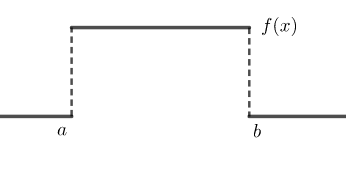
\includegraphics[width=0.4\linewidth]{./Imágenes/aaa.png}
	\end{subfigure}
	\caption{Representación de la función de densidad de una v.a. de distribución uniforme.}
\end{figure}

A veces, es común verla como $f(x) = \frac{1}{b-a}$ para $a<x<b$. Se da por supuesto que, fuera de ese rango, la función es nula.

Para indicar que $X$ tiene una distribución uniforme, lo escribimos como: \[X\sim \U(a,b)\]

\textbf{¿Cuándo la voy a usar?} En algunas situaciones, y en la mayoría de los ejercicios que tendremos que resolver, es muy útil saber que: \[P\left( X \in (c,d) \right)= \frac{d-c}{b-a} \qquad \quad \text{siempre y cuando }(c,d)\subset (a,b)\]

\begin{itemize}
	\item \textbf{Media:} $\displaystyle{\mu = \frac{a+b}{2}}$
	\item \textbf{Varianza:} $\displaystyle{\sigma ^2 = \frac{\left( b-a \right)^2}{12}}$
\end{itemize}

\subsubsection{Distribución exponencial}
En las v.a. con distribución exponencial, nos interesa el \textbf{tiempo que hay que esperar hasta que suceda cierto evento }. Una v.a. $T$ tiene distribución exponencial si su función de densidad es: \[f(t) = \left\{ \begin{matrix}
		\lambda e^{-\lambda t} & \quad t>0           \\[5pt]
		0                      & \quad  \text{resto}
	\end{matrix} \right.\qquad\qquad  \left( \lambda >0 \right)\]

Para indicar que $T$ tiene una distribución exponencial, lo escribimos como: \[T\sim \Exp(\lambda )\]

\begin{itemize}
	\item \textbf{Media:} $\displaystyle{\mu = \frac{1}{\lambda}}\quad $ (tiempo medio de espera)
	\item \textbf{Varianza:} $\displaystyle{\sigma ^2 = \frac{1}{\lambda ^2}}$
\end{itemize}

\subsubsection{Distribución normal}
Una v.a. $X$ tiene distribución normal si su función de densidad es la \textbf{campana de Gauss}: \[f(x) = \frac{1}{\sigma \sqrt{2\pi}}e^{-\frac{1}{2}\left( \frac{x-\mu }{\sigma} \right)^2} \qquad -\infty <x< \infty \]

Sin embargo, no es posible calcular su función de distribución en términos generales.

Para indicar que $X$ tiene una distribución normal, caracterizada por su media y su desviación típica, lo escribimos como: \[X \sim \N(\mu , \sigma ) \]

Además, se suele utilizar la \textbf{distribución normal estándar} $\N(0,1)$, ya que está tabulada. En otras palabras, para realizar los ejercicios utilizaremos una tabla con los valores más utilizados. Sin embargo, en la tabla no aparecen valores negativos de $X$. Eso se debe a que se puede calcular como $\Phi (-x) = 1 - \Phi(x)$.

Cuando nos encontremos con una v.a. $X$ que se distribuya con una normal, lo que debemos hacer es \textbf{tipificarla}. Esto signfica que definiremos otra v.a. $Z$ que modelice a $X$ para que tenga distribución normal.
\[\boxed{X \sim \N(\mu ,\sigma ) \ \longrightarrow \ Z = \frac{X-\mu}{\sigma} \sim \N(0,1)}\]

\section{Desigualdad de Chebyshev}
Sea $X$ una v.a. con media $\mu$ y varianza $\sigma ^2$, entonces para todo $k>0$ se cumple lo siguiente: \[P\left( \abs{X-\mu} < k\sigma \right)\geq 1 - \frac{1}{k^2}\]

\begin{nota}
	Es más fácil comprender la desigualdad de Chebyshev si la reescribimos de esta forma: \[ P\left[ (\mu - k\sigma )< X < (\mu +k\sigma ) \right] \geq 1 - \frac{1}{k^2}\]
\end{nota}


\section{Cuantil}
\subsection*{En v.a. discreta}
Sea $X$ una v.a. discreta, llamaremos \textbf{cuantil de orden} $p$, denotado como $q_p$, al menor valor en el que se cumpla que: \[F_X(x)\geq p \qquad \qquad \left( 0 < p < 1 \right) \]

\subsection*{En v.a. continua}
Sea $T$ una v.a. continua, llamaremos llamaremos \textbf{cuantil de orden} $p$, denotado como $q_p$, al número que verifica: \[P\left( T \leq q_p \right) = \int_{-\infty}^{q_p}{f(x)\dd{x}} = p\]

O, en otras palabras: \[\boxed{F_T(q_p)=p}\]


\section{Percentil}
El percentil es un tipo de cuantil que separa las muestras en 100 grupos diferentes. Para calcular el \textbf{percentil de orden} $n$ de una v.a., basta con saber que: \[P_n = q_{\frac{n}{100}}\]


\chapter{Vectores aleatorios}
\section{Variable aleatoria bidimensional}

Una variable aleatoria bidimensional se puede definir como una transformación tal que:
\[\left( X,Y \right) : \Omega \longrightarrow \mathbb{R}^2\]

De modo que, teniendo el experimento $\omega \in \Omega$, la variable aleatoria bidimensional asigna a cada resultado de dicho experimento un elemento de $\mathbb{R}^2$ que es $\left( X(\omega ),Y(\omega )\right)$.

Esta es \textbf{la misma definición} que para variables aleatorias unidimensionales, pero extrapolada a dos dimensiones. Se podría decir que una variable aleatoria bidimensional está compuesta de dos variables aleatorias unidimensionales, como en un paquete.

\section{Variable aleatoria bidimensional discreta}

La \textbf{función de probabilidad conjunta} de una variable aleatoria bidimensional discreta es una función que proporciona la información esencial de las variables $X$ e $Y$, y se define como:
\[P\left( X=x_i,Y=y_j \right) = P\left( X=x_i \cap Y=y_j \right) \, , \qquad i, j = 1, 2, \dots \] 

A partir de esta función, se pueden calcular las funciones de probabilidad de las variables aleatorias $X$ e $Y$. En este contexto, se les denomina \textbf{funciones de probabilidad marginales}:
\[ P\left( X=x_i \right) = \sum_{j=1}^{\infty} P\left( X=x_i, Y=y_j \right) \, , \qquad i = 1, 2, \dots \]
\[ P\left( Y=x_j \right) = \sum_{i=1}^{\infty} P\left( X=x_i, Y=y_j \right) \, , \qquad j = 1, 2, \dots \]

Es importante observar que la probabilidad del espacio muestral es 1, por lo que se verifica que:
\[ \sum_{i=1}^{\infty}\sum_{j=1}^{\infty} P\left( X=x_i, Y=y_j \right) = 1 \]

\section{Variable aleatoria bidimensional continua}

La \textbf{función de probabilidad conjunta} de una variable aleatoria bidimensional continua es una función que proporciona la información esencial de las variables $X$ e $Y$, y se define como:

\[ P\left( \left( X,Y \right) \in D\right) = \iint_{D}f_{X,Y}(x,y)\dd{y} \dd{x}\]

O, en particular:
\[P\left( a\leq X \leq b, c\leq Y \leq d\right) = \int_{a}^{b}\int_{c}^{d} f_{X,Y}(x,y)\dd{y} \dd{x}\]

Además:
\[\boxed{F_{X,Y}(x,y) = P \left( X\leq x, Y\leq y\right)} = \int_{-\infty}^{x}\int_{-\infty}^{y} f_{X,Y}(\xi , \eta ) \dd{\xi} \dd{\eta}\]

Al igual que antes, la propabilidad del espacio muestral es 1. Por tanto, se verifica que:
\[\int_{-\infty}^{\infty}\int_{-\infty}^{\infty} f_{X,Y}(x,y) \dd{x} \dd{y} = 1\]

Como consecuencia del teorema fundamental del cálculo, se obtiene la siguiente expresión:
\[\pdv[2]{}{x}{y} F_{X,Y}(x,y) = f_{X,Y}(x,y)\]

Las variables aleatorias continuas $X$ e $Y$ tienen funciones de densidad, que en este caso denominaremos \textbf{funciones de densidad marginales}

\section{Independencia de variables aleatorias}
Sea $\left( X,Y\right)$ una variable aleatoria bidimensional, se dice que $X$ e $Y$ son independientes si para cualquiera $A$ y $B$:
\[P\left( X\in A, Y\in B\right) = P\left(X\in A\right)\cdot P\left(Y\in B\right)\]

Si $X$ e $Y$ son independientes, las variables aleatorias definidas a continuación también serán independientes:
\[U=g(X) \qquad \qquad V=h(X)\]

\section{Momentos}

\subsection{Esperanza}

Sea $\left(X,Y\right)$ una variable aleatoria discreta, la \textbf{esperanza} de la variable aleatoria $g\left(X,Y\right)$ es:
\[E\left[g\left(X,Y\right)\right] = \sum_{x_i,y_j\in S}g\left(x_i,y_j\right)P\left(X=x_i, Y=y_j\right)\]

Sea $\left(X,Y\right)$ una variable aleatoria continua, y análoga a la definición anterior, la esperanza de la variable aleatoria $g\left(X,Y\right)$ es:
\[E\left[g\left(X,Y\right)\right] = \int_{-\infty}^{\infty}\int_{-\infty}^{\infty}g\left(x,y\right)f_{X,Y}(x,y)\dd{x} \dd{y}\]

La esperanza es un operador \textbf{lineal}.

\subsection{Covarianza}

La covarianza se usa para \textbf{medir el grado de correlación} entre las variables $X$ e $Y$. Se define como:
\[\Cov \left( X,Y \right) = E \left[\left(X-E\left[X\right]\right) \cdot \left(Y - E\left[Y\right]\right)\right]\]

Sin embargo, \textbf{la forma habitual} de calcular la covarianza es la siguiente:
\[\Cov \left( X,Y \right) = E\left[X\cdot Y\right] - E\left[X\right]E\left[Y\right]\]

Para dos números $a,b \in \mathbb{R}$, se cumple que:
\[\Cov \left( aX,bY \right) = ab\Cov \left( X,Y \right)\]

Esta propiedad puede dificultar algunas operaciones. Por eso, se define el \textbf{coeficiente de correlación lineal} mediante la normalización de la covarianza:
\[\rho \left(X,Y\right) = \frac{\Cov \left( X,Y \right)}{\sigma _X \sigma _Y} \]

Es importante recalcar que $\rho \left( aX,bY \right) = \rho \left( X,Y \right) $. Además, se verifica que:
\[-1\leq \rho \left( X,Y \right) \leq 1 \]

Las variables aleatorias $X$ e $Y$ son \textbf{incorreladas} si $\rho \left( X,Y \right)=0$.

Si las variables aleatorias $X$ e $Y$ son independientes, son incorreladas. Por lo tanto:
\[X \text{ e } Y \text{ son independientes} \ \Longrightarrow \left\lbrace \begin{matrix*}[l]
	E \left[ X \cdot Y \right] = E \left[ X \right] E \left[ Y \right] \\[5pt] 
	\Cov \left( X,Y \right) = 0 \\[5pt] 
	\rho \left( X,Y \right) = 0
\end{matrix*} \right. \] 

\subsection{Notación matricial}
El \textbf{vector de medias} se define como:
\[ \vec{m} = \left[ 
\begin{matrix}
	E \left[ X \right]\\ 
	E \left[ Y \right]
\end{matrix} \right] \]

La \textbf{matriz de covarianza} se define como:
\[M=\left[ 
\begin{matrix}
	\Var \left( X \right)& \Cov \left( X,Y \right)\\ 
	\Cov \left( X,Y \right)& \Var \left( Y \right)
\end{matrix} \right]\]

\section{Variable aleatoria multidimensional}

Prácticamente todas las definiciones mostradas para dos variables aleatorias se pueden generalizar para $n$ variables aleatorias.

Una variable aleatoria $n$-dimensional se define como una aplicación:
\[\left( X_1,X_2,\dots , X_n \right):\Omega \longrightarrow \mathbb{R}^n\]
Esta variable aleatoria asigna a cada resultado del excperimento $\omega \in \Omega$ un elemento\\ $\left( X_1(\omega ), X_2(\omega ) \dots X_n (\omega )\right)\in \mathbb{R}^n$

Para cualquiera de las operaciones lineales, resulta apropiada la notación por columnas:
\[\vec{X} = \left[ 
\begin{matrix}
	X_1\\ 
	X_2\\ 
	\vdots \\ 
	X_n
\end{matrix} \right]\]

Por lo tanto, escribiremos el vector de medias como:
\[\vec{m}_{\vec{X}} = E \left[ \vec{X} \right]= \left[ 
\begin{matrix}
	E \left[ X_1 \right]\\ 
	E \left[ X_2 \right]\\ 
	\vdots \\ 
	E \left[ X_n \right]
\end{matrix} \right] \]

Y la matriz de covarianzas como:
\[ M_{\vec{X}} = \left[ 
\begin{matrix}
	\Var \left( X_1 \right) & \Cov \left( X_1, X_2 \right) & \cdots & \Cov \left( X_1, X_n \right)\\ 
	\Cov \left( X_1, X_2 \right) & \Var \left( X_2 \right) & \cdots & \Cov \left( X_2, X_n \right)\\ 
	\vdots & \vdots & \ddots & \vdots \\
	\Cov \left( X_1,X_n \right) & \Cov \left( X_2, X_n \right) & \cdots & \Var \left( X_n \right)
\end{matrix} \right]\]

\subsubsection{Linealidad}
Si se realiza una combinación lineal con las variables aleatorias $\left( X_1,X_2, \dots , X_n \right)$ se obtiene una variable aleatoria:
\[ Y = a_1X_1 + a_2X_2 + \dots + a_nX_n \]

Podemos expresar la variables aleatoria $Y$ de la siguiente forma:
\[ Y = A \vec{X}, \qquad A = \left[ 
\begin{matrix}
	a_1 & a_2 & \cdots & a_n
\end{matrix} \right] \]

Por la linealidad de la \textbf{esperanza}, tenemos que:
\[ E \left[ Y \right] = a_1E \left[ X_1 \right] + a_2 E \left[ X_2 \right] + \dots + a_n E \left[ X_n \right] \]

La \textbf{varianza} de $Y$ será:
\[ \Var \left( Y \right) = A \times M_{\vec{X}} \times A ^{\top} \]

Donde $A ^{\top} $ es la matriz traspuesta de $A$. Se puede generalizar este resultado para $m$ combinaciones lineales. Suponiendo que:
\[ \vec{Y} = A \vec{X} + \vec{v} \]
 
Donde $A$ es una matriz de dimensión $m \times n$ y $\vec{b}$ es un vector columna, entonces la variables aleatoria $m$-dimensional $\vec{Y}$ tiene un vector de medias $\vec{m}_{\vec{Y}}$ y una matriz de covarianza $M_{\vec{Y}}$ tales que:
\[ \vec{m}_{\vec{Y}} = A \vec{m}_{\vec{X}} + \vec{b} \, ; \qquad \qquad \vec{m}_{\vec{Y}} = A \vec{m}_{\vec{X}} A ^{\top} \]

\section{Distribución multinomial}

Si se realizan $n$ pruebas de Bernoulli, la variable aleatoria bidimensional $\left( X_1, X_2 \right)$ definida por:
\[ \begin{matrix*}[l]
	X_1 \equiv \text{número de éxitos}\\[5pt] 
	X_2 \equiv \text{número de fracasos}
\end{matrix*} \]

Esta variable solo podrá tomar los valores $\left( n_1, n_2 \right)$ con $n_1 = 0,1, \dots , n$ y $n_2 = n - n_1$. Para estos valores:
\[ P \left( X_1 = n_1, X_2 = n_2 \right) = \frac{n!}{n_1!n_2!} p_1^{n_1} p_2^{n_2}\]

Donde $p_1 = p$ es la probabilidad de éxito y $p_2 = 1-p$ es la probabilidad de fracaso.

Un caso intereseante es aquel en el que en cada una de las $n$ pruebas se puedan obtener $k$ posibles resultados $A_1,A_2, \dots ,A_k$ con probabilidades $p_1,p_2, \dots ,p_k$, donde necesariamente $p_1 +p_2 + \dots + p_k = 1$. La variable $n$-dimensional $\left( X_1, \dots X_k \right)$ definida por:
\[ \begin{matrix*}[l]
	X_1 \equiv \text{número de veces que se obtiene }A_1\\[5pt] 
	X_2 \equiv \text{número de veces que se obtiene }A_2\\[5pt] 
	\ \, \vdots \\[5pt] 
	X_k \equiv \text{número de veces que se obtiene }A_k
\end{matrix*} \]

solo puede tomar valores $\left( n_1, n_2, \dots , n_k \right)$ con $n_1,\dots ,n_k=0,1,\dots ,n$ y $n_1 + \dots + n_k = 1$. Para estos valores se tiene que:
\[ P \left( X_1=n_1, \dots , X_k = n_k \right) = \frac{n!}{n_1!n_2!\dots n_k!} p_1^{n_1} \dots p_k^{n_k} \]

Se dice que es $\left( X_1,\dots ,X_k \right)$ sigue una distribución multinomial de parámetros $n,p_1,p_2,\dots p_k$, y se denota como:
\[ \left( X_1,\dots ,X_k \right) \sim \Mult \left( n,p_1,p_2,\dots p_k \right) \]

\section{Distribución normal n-dimensional}

Un vector aleatorio $ X = \left( X_1, \dots , X_n \right) $ sigue una distribución normal si la denominada función de densidad
\[ f_{X_1,\dots , X_n}\left( x_1, \dots , x_n \right) = \frac{\partial ^n}{\partial x_1 \dots \partial x_n}F_{X_1, \dots , X_n} \left( x_1, \dots , x_n \right)\]
es igual a
\[ \frac{1}{\abs{M_{\vec{X}}}^{\frac{1}{2} } \left( 2 \pi  \right) ^{\frac{n}{2}}} e^{-\frac{1}{2}\left( \vec{X} - \vec{m}_{\vec{X}} \right) ^{\top} M_{\vec{X}}^{-1} \left( \vec{X} - \vec{m}_{\vec{X}} \right) }\]

donde $M_{\vec{X}}$ es la matriz de covarianzas y $\vec{m}_{\vec{X}}$ es el vector de medias.

\section{Teorema central del límite}

Vamos a utilizar la definición de este teorema que nos será útil para resolver los ejercicios. La definición completa es [FALTA REFERENCIA].

Sean $X_1,\dots , X_n$ variables aleatorias independientes e idénticamente distribuidas, cada una con media $\mu$ y varianza $\sigma ^2$.

El \textbf{teorema central del límite} afirma que si $n$ es grande la suma $S_n$ tiene aproximadamente distribución normal de media $n\mu$ y desviación típica $\sigma \sqrt{n}$ (varianza $n\sigma ^2$), siendo esta suma:
\[ S_n = X_1 + X_2 + \dots + X_n \]

Equivalentemente, la \textbf{variable normalizada} $\frac{S_n-n\mu}{\sigma \sqrt{n}}$ tiene aproximadamente distribución normal de media 0 y varianza 1.

\section{Chi cuadrado y la t de Student}

Sean $Z_1,\dots ,Z_n$ variables aleatorias independientes con distribución normal estándar, $Z_i \sim N \left( 0,1 \right)$, con $i=1,\dots ,n$.

La distribución de probabilidad que sigue la variable aleatoria
\[ X=Z_1^2+\dots +Z_n^2 \]
se denomina chi-cuadrado con $n$ grados de libertad. Se denota $X\sim \chi _n^2$. La distribución $\chi _n^2$ es positiva. Su media y su varianza son:
\[ E (X) = n \, ; \qquad \qquad \Var \left( X \right)=2n \]

Sea $X\sim \chi _n^2$, y $Z$ una variable aleatoria con distribución normal estándar, $Z\sim \N(0,1)$, independiente de $X$. La distribución de probabilidad que sigue la variable aleatoria
\[Y=\frac{Z}{\sqrt{X/n}}\]
se denomina $t$ de Student con $n$ grados de libertad. Se denota $Y\sim t_n$. La $t$ de Student tiene una función de densidad simétrica muy similar, casi igual si $n$ es grande, a la de una normal $\N(0,1)$. La principal diferencia es la varianza, que vale:
\[ \Var \left( Y \right)=\frac{n}{n-2}  \]

\chapter{Inferencia estadística}

\section{Estadística descriptiva de una variable: momentos, cuantiles, box-plot, histograma, función de distribución empírica y cálculo de proporciones}
\section{Muestra aleatoria. Media muestral y varianza muestral. Estimación paramétrica}

\section{Intervalos de confianza para la media y para proporciones poblacionales}

\section{Contraste de hipótesis. Nivel de significación y p-valor}



\chapter{Procesos estocásticos}

\section{Definición de proceso estocástico}
Un proceso estocástico es una familia de variables aleatorias definidas sobre un espacio probabilístico.

Sea $X(t)$ una variable aleatoria para cada instante de tiempo $t\in T$; un \textbf{proceso estocástico} es una familia de variables aleatorias que describe la evolución a lo largo del tiempo de algún proceso físico.

Otro punto de vista:

Sea $E$ un experimento aleatorio cuyo espacio probabilístico asociado sea $(\Omega , S, P)$. Un \textbf{proceso estocástico} o proceso aleatorio es un conjunto de funciones temporales $x(t,\omega )$, cada una correspondiente a un punto particular $\omega$ del espacio muestral $\Omega$. Así, asociado a cada resultado específico $\omega$, tenemos una función específica $x(t,\omega )$, a la que llamaremos una realización del proceso.

Denotaremos el proceso mediante: $X_t\equiv X(t) \equiv X(t,\omega )$, donde $t$ es el tiempo y $\omega$ una variable que representa un resultado en el espacio muestral $\Omega$.

Normalmente, un proceso estocástico será denotado como $x(t)$.

\section{Procesos estocásticos en tiempo continuo}
\textbf{Primer ejemplo.}

Tiramos un dado. Si se obtiene 1, 2 ó 3, entonces:
\[X(t) = t\]
Si se obtiene 4 ó 5, entonces:
\[X(t) = 2t\]
Si se obtiene un 6, entonces:
\[X(t) = 3t\]

Esto se puede modelizar de la siguiente manera:
\[X(t) = A\cdot t\]
De modo que la probabilidad de $A$ será:
\begingroup
\renewcommand{\arraystretch}{1.2}
\begin{center}
	\begin{tabular}{r || c | c | c}
		$A$ & 1 & 2 & 3 \\ \hline
		$P(A)$ & $\sfrac{1}{2}$ & $\sfrac{1}{3}$ & $\sfrac{1}{6}$
	\end{tabular}
\end{center}
\endgroup

\textbf{Segundo ejemplo.}

La señal $X(t) = \cos\left( t+\phi \right)$, donde la fase $\phi$ es desconocida, se puede considerar como un proceso estocástico, donde $\phi$ es una variable aleatoria con distribución uniforme en el intervalo $[0, 2\pi )$

\section{Procesos estocásticos en tiempo discreto}

Habitualmente, la notación para los procesos estocásticos es $X(n)$, donde $n$ solo puede tomar valores discretos.

\subsection{Procesos de Bernoulli y Binomial}

Se realizan pruebas de Bernoulli siendo $p$ la probabilidad de éxito $(E)$.

El \textbf{proceso de Bernoulli} asociado es:
\[ I(n)= \left\lbrace 
\begin{matrix*}[l]
	1, & \text{si en la prueba } n \text{-ésima se obtiene }E\\ 
	0, & \text{en otro caso}
\end{matrix*} \right. \]

El \textbf{proceso binomial} asociado es:
\[ B(n) = I(1), \dots , I(n) \]
que da el número de éxitos obtenido hasta la $n$-ésima prueba.

\subsection{Caminata aleatoria simétrica} \label{sec:caminata_aleatoria_simetrica}

Asociado a las pruebas de Bernoulli con probabilidad de éxito $p=\frac{1}{2}$, consideramos el proceso:
\[ D(n) = \left\lbrace 
\begin{matrix*}[l]
	\phantom{-} 1, & \text{si en la prueba } n \text{-ésima se obtiene }E\\ 
	-1, & \text{en otro caso}
\end{matrix*} \right. \]

Entonces, el proceso $S(n)$ se denomina \textbf{caminata aleatoria}.
\[ S(n) = D(1)+D(2)+\dots +D(n) \]

Se le llama así porque la definición de $S(n)$ implica que:
\[ S(n) = S(n-1) + D(n) \]
Y esto significa que, en el instante de tiempo $n$, la probabilidad de subir una unidad y la probabilidad de bajar una unidad, ambas son de $p=\frac{1}{2}$. 

\section{Distribuciones de primer orden}

Las funciones que describen las distribuciones de probabilidad son de $n$-ésimo orden si se fija un número $n$ de valores fijos de $t$.

Para un tiempo $t$ fijo (funciones de distribución de primer orden), un proceso estocástico $X(t)$ es, en realidad, una variable aleatoria. Su función de distribución se denota como:
\[ F \left( x;t \right) = P \left( X(t) \leq x \right) \]

Si trabajamos en tiempo continuo, la función de densidad será:
\[ f(x;t) = \dv{}{x} F(x;t) \]

Si trabajamos en tiempo discreto, y tomando valores $n\in \mathbb{Z}$, la función de densidad será:
\[ f \left( n;t \right) = P \left( X(t) = n \right) \]

La media del proceso $X(T)$ es función del tiempo:
\[ \mu _X (t) = E \left[ X(t) \right] \]

\subsection{Procesos de Bernoulli y Binomial}

La distribución de primer orden del proceso de Bernoulli $I(n)$ viene dada por:
\[ P \left( I(n) = 1 \right) = p \, \qquad \qquad P \left( I(n) = 0 \right) = 1-p \]
donde $p$ es la probabilidad de éxito. La del proceso binomial $B(n)$ asociado viene dada por:
\[ B(n)\sim \BN (n,p) \]

Las medias de estos procesos son:
\[ \mu _1 (n) = p \qquad \text{y} \qquad  \mu _B (n) = np\]

\section{Distribuciones de segundo orden}

Para dos valores de tiempo fijos, $t_1$ y $t_2$, la variable $\left( X(t_1), X(t_2) \right)$ es una variable aleatoria bidimensional.

Su función de distribución es:
\[ F \left( x_1,x_2;t_1,t_2 \right) = P \left( X(t_1) \leq x_1, X(t_2) \leq x_2 \right) \]

Si trabajamos en tiempo continuo, la función de densidad será:
\[ f \left( x_1,x_2;t_1,t_2 \right) = \pdv{}{x_1}{x_2}F \left( x_1,x_2;t_1,t_2 \right)  \]

Si trabajamos en tiempo discreto, la función de densidad:
\[ f \left( n,m;t_1,t_2 \right) = P \left( X(t_1) = n, X(t_2) \right) \]

De forma análoga se podrán sintetizar las funciones de densidad y distribución de cualquier orden.

Se define la \textbf{autocovarianza} como la función que proporciona la covarianza entre $X(t_1)$ y $X(t_2)$:
\[ C_X \left( t_1,t_2 \right)= \Cov \left[  X(t_1), X(t_2)\right] \]

Es interesante ver que:
\[ C_X \left( t_1,t_2 \right) = E \left[ X(t_1)X(t_2) \right] - E \left[ X(t_1)\right]\left[ X(t_2)\right] = \mathcal{R}_X \left( t_1,t_2 \right) - \mu (t_1)\mu (t_2)\]

Donde $\mathcal{R}_X$ es la \textbf{autocorrelación} del proceso.
\[\mathcal{R}_X \left( t_1,t_2 \right) = E \left[ X(t_1)X(t_2) \right]\]

En particular:
\[ \Var \left( X(t) \right) = C_X(t,t) = \mathcal{R}_X(t,t)-\mu ^2(t) \]

Se denomina \textbf{coeficiente de autocorrelación} a:
\[ \rho _X(t_1,t_2) = \frac{C_X \left( _1,t_2 \right)}{\sqrt{\Var \left( X(t_1) \right) \Var \left( X(t_2) \right)}} \]

\section{Independencia}

Se dice que el proceso $X(t)$ y la variable aleatoria $A$ son independientes si para cualquier tiempo $t_1,\dots ,t_n$ las variables aleatorias $A, X(t_1), \dots ,X(t_n)$ también son independientes.

Se dice que dos procesos $X(t)$ e $Y(t)$ son independientes si para cualesquiera tiempos $t_1, \dots , t_n$ y $t_1', \dots , t_n'$ las variables aleatorias $\left[ X(t_1), \dots , X(t_n) \right]$ y $\left[ Y(t_1'), \dots , Y(t_n') \right]$ son también independientes.

\section{Proceso de Poisson}

Suponemos un suceso que ocurre en ciertos instantes de tiempo.

Sea $N(t)$ el número de sucesos ocurridos hasta $t$.
\[ N(t) \equiv \text{nº de sucesos ocurridos en }(0,t] \]

Nótese que el número de sucesos ocurridos en un intervalo $(a,b)$ es $N(b)-N(a)$

Se define la \textbf{tasa} como el número medio de sucesos que ocurren por unidad de tiempo.

Si los sucesos ocurren de forma completamente aleatoria en el tiempo la tasa es $\lambda$, entonces se verifican las siguientes condiciones:
\begin{enumerate}
	 \item $N(0)=0$
	 \item El número de sucesos que se producen en intervalos de tiempo disjuntos son independientes. Si $(a,b) \cap (c,d) = \emptyset$ entonces $N(b)-N(a)$ y $N(d)-N(c)$ son variables aleatorias independientes.
	 \item El número de sucesos que se producen en un intervalo no depende de la situación del intervalo, sino únicamente de su duración. Las variable aleatoria $N(t+\tau ) - N(t)$ y la variable aleatoria $N(\tau )$ tienen la misma función de probabilidad.
	 \item Para cada valor fijo de $t$, la variable $N(t)$ tiene distribución de Poisson de media $\lambda t$.
\end{enumerate}

Si estas condiciones se cumplen, se dice que $N$ es un proceso de Poisson de tasa $\lambda $.

Según la cuarta condición, las distribuciones de de primer orden son de $\Poisson \left( \lambda t \right)$:
\[ P \left[ N(t) = k \right] = \frac{\left( \lambda t \right)^k}{k!}e^{-\lambda t} \, , \qquad k = 0, 1, \dots \]

La media del proceso $N$ es:
\[ E \left[ N(T) \right] = \lambda t\]

Por esta definición, la tasa $\lambda$ es el número medio de sucesos ocurridos por unidad de tiempo.

El \textbf{tiempo de espera} $T$ hasta que ocurra un suceso tiene distribución exponencial de media $\frac{1}{\lambda}$. Por ello, su función de distribución es:
\[ F_T(t) = 1-P \left( N(t) =0 \right) = 1 - e^{-\lambda t} \, , \qquad t>0\]

\section{Procesos normales}
Un proceso $X(t)$ es normal o Gaussiano cuando para valores de tiempo fijos $t_1, \dots , t_n$ la variable aleatoria $\left[ X(t_1), \dots , X(t_n) \right]$ tiene distribución normal.

Este tipo de procesos es el más utilizado para modelar el ruido en el estudio del procesado de señales.

Al igual que en ocasiones anteriores, para el análisis de procesos normales resultará útil la siguiente propiedad. Para $A\in \mathcal{M}_{m\times n}$ y $B\in \mathcal{M}_{m\times 1}$, la variable:
\[ \vec{Y} = A \vec{X} + \vec{B} \]
tiene distribución normal con vector de medias
\[ \vec{m}_{\vec{Y}}= A \vec{m}_{\vec{X}} + B\]
y matriz de covarianzas
\[ M_{\vec{Y}} = A M_{\vec{X}} A ^{\top} \]

En particular, si tenemos un vector $a=\left[ 
\begin{matrix}
	a_1\\
	\vdots \\
	a_n
\end{matrix} \right]$, y definimos la variable $Y$ como:
\[ \vec{Y}= a_1X(t_1) + \dots + a_nX(t_n) = \vec{a}^{\top}  \vec{X}\]

Entonces, $Y$ tiene distribución normal cuya media y cuya varianza son:
\[ \mu _{\vec{Y}} = \vec{a} ^{\top} \vec{m} \, , \qquad \sigma ^2 _{\vec{Y}} = \vec{a} M \vec{a}^{\top} x\]

\section{Proceso de Wiener}

Un proceso de Wiener es un proceso estocástico normal (al que llamaremos $X(t)$) con media $\mu _X (t) = 0$ y autocovarianza:
\[ C_X \left( t_1, t_2 \right) = \alpha \min\left( t_1, t_2 \right)\]

En realidad, el proceso de Wiener se parece mucho a una \hyperref[sec:caminata_aleatoria_simetrica]{caminata aleatoria simétrica}. Cada $h$ segundos (siendo $h$ un número muy pequeño) se salta hacia arriba o abajo con probabilidad $\frac{1}{2}$ una distancia de $\sqrt{\alpha h}$. 

\section{Procesos estacionarios}

Si las causas de la aleatoreidad no varían con el tiempo, entonces hablamos de que los procesos son \textbf{estacionarios}.

\begin{itemize}
	 \item Un proceso es estacionario \textbf{en sentido estricto} si la distribución de probabilidad de cualquier orden no depende del origen de tiempos.
	 \item Un proceso es estacionario \textbf{en sentido amplio} si tiene media constante y su autocorrelación depende únicamente de la distancia entre los tiempos $\tau$ y se denota:
	 \[ \mu _X = \mu _X(t) \, , \qquad \mathcal{R}_X \left( \tau \right) = \mathcal{R}_X \left( t, t+ \tau \right) \]
	 La autocovarianza tampoco depende del tiempo, y es:
	 \[ C_X(\tau ) = \mathcal{R}_X(\tau )-\mu_X^2 \]
\end{itemize}

Es importante ver que un proceso estacionario en sentido estricto también es estacionario en sentido amplio. Sin embargo, no siempre se cumple a la inversa.

Además, todos los procesos normales son estacionarios en sentido estricto. Aunque en estos casos se los denomina estacionarios, a secas.

\section{Sistemas lineales}

La \textbf{densidad espectral} de un proceso estacionario en sentido amplio como la transformada de Fourier de la autocorrelación:
\[ S_X(\omega ) = \int_{-\infty}^{\infty} \mathcal{R}_X (\tau )e^{-j\tau \omega }\dd{\omega} \]

La densidad espectral es una función real, positiva y par.

Además, aplicando la transformada inversa de Fourier podemos obtener:
\[ \mathcal{R}_X(\tau )=\frac{1}{2\pi}\int_{-\infty}^{\infty}S_X(\omega )e^{j\tau \omega} \dd{\omega}\]

Para el caso particular de $\tau = 0$, tenemos que:
\[ \mathcal{R}_X(0)=\frac{1}{2\pi}\int_{-\infty}^{\infty}S_X(\omega )\dd{\omega}\]

Llamaremos $H(\omega )$ a la función de transferencia del sistema, que es la transforma de Fourier de la respuesta al impulso $h(t)$ (más información en los apuntes de \href{\detokenize{https://github.com/Javiolonchelo/ApuntesTeleco_2/blob/main/Primer%20Semestre/Señales%20y%20Sistemas/Señales_y_Sistemas.pdf}}{Señales y Sistemas}).

Esta fórmula expresa la potencia media del ruido en función de la densidad espectral.

Si la entrada a un sistema $X(t)$ es un proceso estacionario en sentido amplio, entonces la salida $Y(t)$ es un proceso también estacionario en sentido amplio cuya media es:
\[ \mu _Y = H(0)\mu _X \]

Y cuya densidad espectral es:
\[ S_Y(\omega )= \abs{H(\omega )}^2 S_X(\omega )  \]

Estas fórmulas sirven para calcular medias y autocorrelaciones de señales filtradas.

Si la entrada $X(t)$ es un proceso normal, la salida $Y(t)$ también lo será, con las características que acabamos de describir.

\chapter{Prácticas con software estadístico}


\section{Modelos de distribución de probabilidad más comunes}

\section{Estadística descriptiva}

\section{Muestreo. Estimación puntual}

\section{Estimación por intervalos de confianza}

\section{Contraste paramétrico}

%%% FIN DE LOS APUNTES %%%

%%% BIBLIOGRAFÍA %%%
% Por defecto, se encuentra desactivada. Esto disminuye el tiempo de procesado. Se puede activar cuando se vaya a exportar el PDF definitivo

%\newpage
%\phantomsection
%\label{sec:bibliografia_final}
%\renewcommand{\refname}{Bibliografía}
%\addcontentsline{toc}{section}{Bibliografía}
%\bibliography{bibliografia} % Nombre del archivo (sin ".bib")
%\bibliographystyle{bababbrv} 

\end{document}
